\documentclass{article}
\usepackage[utf8]{inputenc}
\usepackage{amsmath}
\usepackage{graphicx}

\title{Week One Notes}
\author{Jasper Albert Nri}
\date{September 2021}

\begin{document}

\maketitle

\section*{Introduction}
\begin{enumerate}
    \item First
    $$e^{i\pi}+1=0$$
    
    \item Second
    $$e = \lim_{n\to\infty}\left(1+\frac{1}{n}\right)^n = \lim_{n\to\infty}\frac{n}{\sqrt[n]{n!}}$$ 
    
    \item Third
    $$ e = \sum_{n=0}^{\infty} \frac{1}{n!} $$
    $$ e = 2+\frac{1}{1+\frac{1}{2+\frac{2}{3+\frac{3}{4+\frac{4}{5+\ddots}}}}}$$
    % $$$$
    
    \item Fourth
    $${(a+b)^2 = a^2 +2ab + b^2}$$
    $${(a-b)^2 = a^2 - 2ab + b^2}$$
    $${(a+b)(a-b) = a^2 -  b^2}$$
    $${(x+a)(x+b) = x + (a+b)x + ab}$$
    $${(a+b+c)^2 = a^2+b^2+c^2+2ab+2bc+2ca}$$
    $${(a+b)^3 = a^3 + 3a^2b + 3ab^2 +b^3}$$
    $${(a-b)^3 = a^3 - 3a^2b + 3ab^2 -b^3}$$
    
\end{enumerate}
\section*{Formulas}
$$\int_a^bf(x)dx$$
$$\iiint f(x,y,z)dxdydz$$

Algebra

$$\vec{v}=<v_1, v_2, v_3>$$
$$\vec{v}\cdot \vec{w}$$

Matrices
$$
\begin{bmatrix}
1 & 2 & 3\\
4 & 5 & 6\\
\end{bmatrix}$$


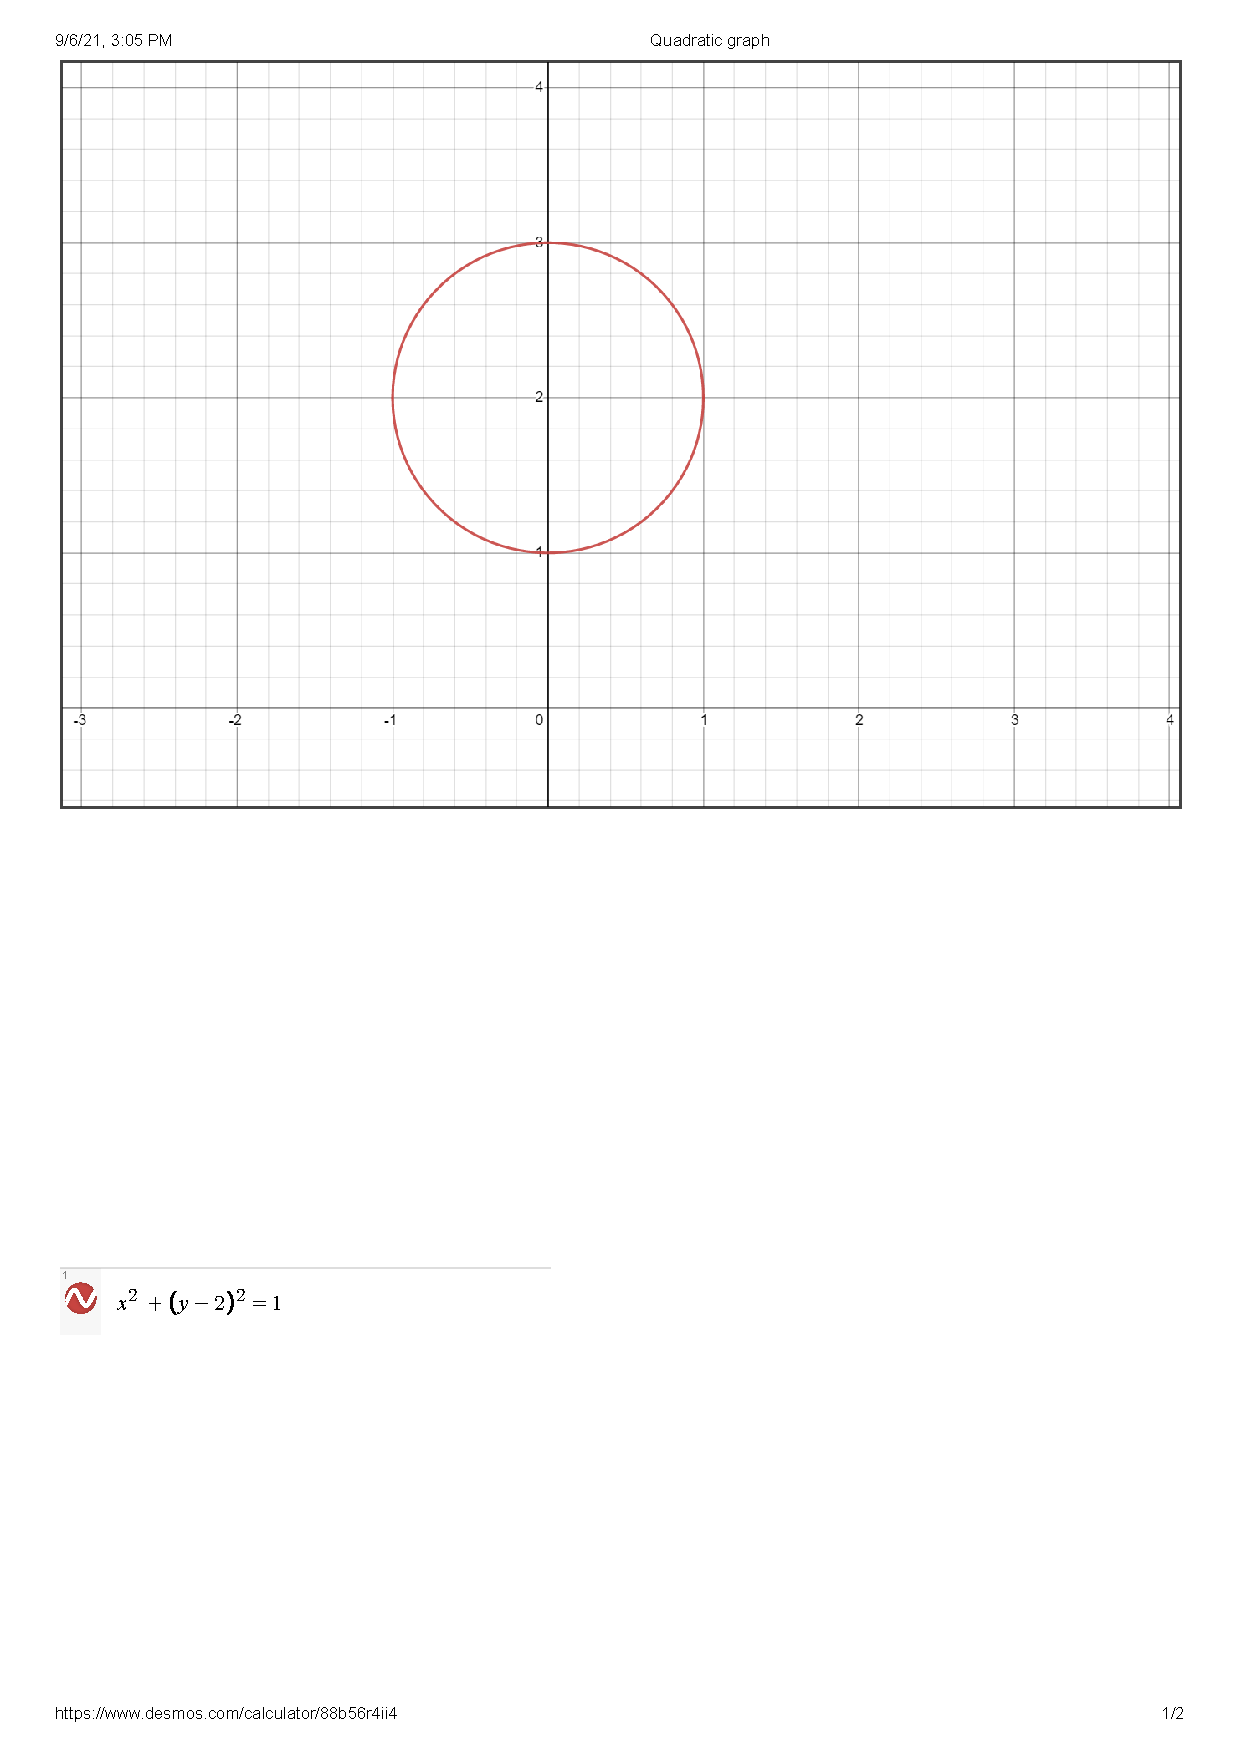
\includegraphics[scale = 0.5]{Quadratic-graph}

% $$$$
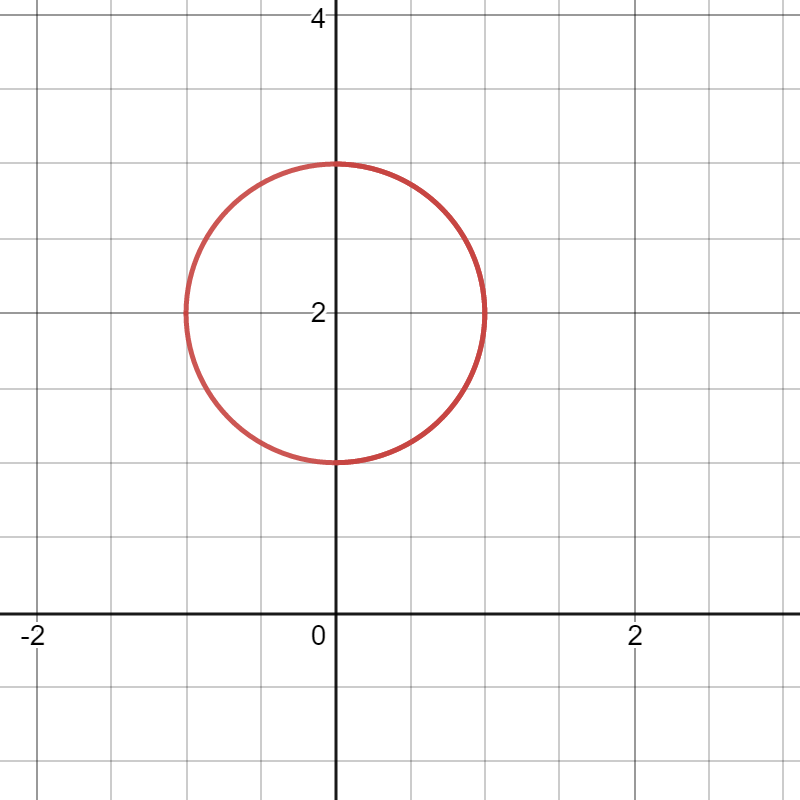
\includegraphics[scale = 0.5]{desmos-graph}
\end{document}